\subsection{UC 21 - Eliminazione evento} \label{sec:UC21}
    \begin{itemize}
        \item \textbf{Attore principale}: MUA;
        \item \textbf{Descrizione}: il MUA deve poter eliminare un evento dal sistema;
        \item \textbf{Precondizioni}: l’account che il MUA gestisce è registrato nel sistema, ha un connessione aperta con il sistema ed è autenticato;
        \item \textbf{Postcondizioni}: il sistema elimina l'evento con l'identificativo fornito dal MUA;
        \item \textbf{Scenario principale}:
            \begin{enumerate}
                \item il MUA invia l'id dell'evento da eliminare al sistema (\hyperref[sec:UC21.1]{UC 21.1});
                \item il sistema elimina l'evento;
            \end{enumerate}
        \item \textbf{Inclusioni}: nessuna;
        \item \textbf{Generalizzazioni}: nessuna;
        \item \textbf{Estensioni}: nessuna.
    \end{itemize}

\begin{figure}[h]
    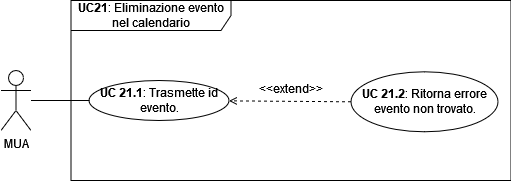
\includegraphics[width=0.85\textwidth]{sections/uc_imgs/UC21.png}
    \centering
    \caption{Diagramma sotto-casi UC 21}
\end{figure}

\subsubsection{UC 21.1 - Trasmette id evento} \label{sec:UC21.1}
    \begin{itemize}
        \item \textbf{Attore principale}: MUA;
        \item \textbf{Descrizione}:  il MUA invia l'id dell'evento da eliminare al sistema;
        \item \textbf{Precondizioni}: il MUA sta usando la funzionalità di eliminazione di un evento;
        \item \textbf{Postcondizioni}:  il sistema conosce l'id dell'evento da eliminare;
        \item \textbf{Scenario principale}:
            \begin{enumerate}
                \item il MUA invia l'identificativo dell'evento da eliminare al sistema;
            \end{enumerate}
        \item \textbf{Inclusioni}: nessuna;
        \item \textbf{Generalizzazioni}: nessuna;
        \item \textbf{Estensioni}:
            \begin{enumerate}[label=\alph*.]
                \item il sistema non riesce a eliminare l'evento perché non è stato trovato:
                \begin{enumerate}[label=\arabic*.]
                    \item il sistema ritorna un errore al MUA di evento non trovato (\hyperref[sec:UC21.2]{UC 21.2}).
                \end{enumerate}
            \end{enumerate}
    \end{itemize}


    \subsubsection{UC 21.2 - Ritorna errore evento non trovato} \label{sec:UC21.2}
    \begin{itemize}
        \item \textbf{Attore principale}: MUA;
        \item \textbf{Descrizione}: il sistema non riesce a eliminare l'evento perché l'evento non è stato trovato;
        \item \textbf{Precondizioni}: il MUA ha inviato l'id dell'evento da eliminare;
        \item \textbf{Postcondizioni}: il sistema non elimina l'evento, il MUA è stato notificato dell'errore;
        \item \textbf{Scenario principale}:
            \begin{enumerate}
                \item il sistema non trova l'evento con l'identificativo fornito dal MUA;
                \item il sistema non elimina l'evento e notifica il MUA dell'errore;
            \end{enumerate}
        \item \textbf{Inclusioni}: nessuna;
        \item \textbf{Generalizzazioni}: nessuna;
        \item \textbf{Estensioni}: nessuna.
    \end{itemize}

